\documentclass{article}

\usepackage[utf8]{inputenc}
\usepackage[dvipsnames]{xcolor}
\usepackage{lmodern}
\usepackage{graphicx}
\usepackage{longtable}
\usepackage{tabularx}
\graphicspath{ {./images/} }
\usepackage{imakeidx}
\makeindex[columns=3, title=Alphabetical Index, intoc]

\usepackage{tabularx}
\usepackage{amsmath}
\usepackage{paralist}
\usepackage{enumitem}
\usepackage{hyperref} %\usepackage[hidelinks]{hyperref} %per togliere bordi rossi
\usepackage{makecell}
\usepackage{caption}
\usepackage[maxfloats=256]{morefloats}
\maxdeadcycles=1000

\usepackage[official]{eurosym}
\DeclareUnicodeCharacter{20AC}{\euro{}}

\author{Agosta, Belli, Emili, Giacchini, Luciani}

\begin{document}

\begin{center}
    \sffamily{\fontsize{50}{48} \selectfont \textcolor{red}{Nexi}\textcolor{green}{Fy}}
\end{center}

\begin{center}
    \itshape{\fontsize{20}{48} \selectfont streaming to your pocket}
\end{center}

\bigskip\bigskip\bigskip

\begin{flushleft}
    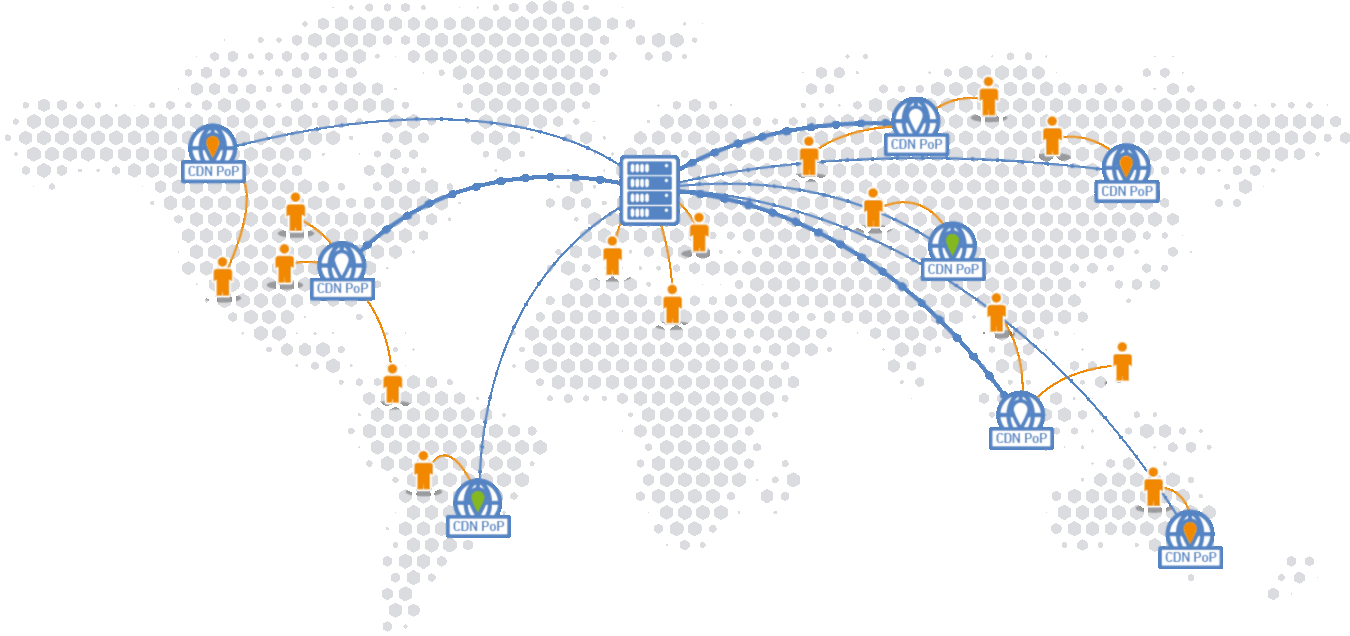
\includegraphics[scale=1]{../images/worldCDN.png}
\end{flushleft}

\bigskip\bigskip\bigskip

\begin{center}
    \itshape{\fontsize{30}{48} \selectfont Modello degli Use-Case}
\end{center}

\newpage
\printindex

\newpage
\section{\itshape{Modello degli Use-Case}}
\setlength{\arrayrulewidth}{.5mm}
\setlength{\tabcolsep}{5pt}
\renewcommand{\arraystretch}{2}
\renewcommand{\labelenumii}{\theenumii}
\renewcommand{\theenumii}{\theenumi.\arabic{enumii}.}

\subsection{Introduzione}
La seguente sezione mira all'identificazione dei casi d'uso presenti nel progetto. Di seguito vengono identificati oltre ai casi d'uso, anche gli attori coinvolti nel loro utilizzo.
Lo scopo principale del documento, è quello di avere un riferimento sui casi d'uso leggibile da chiunque, anche a personale non interno al progetto. Questo è utile al fine di permettere a tutti una comprensione e quindi una discussione sui casi d'uso.

\subsection{Legenda}
\large{\textbf{Attori}} \\
\begin{itemize}[]
	\item \textbf{ID}: rappresenta l'identificatore univoco di un attore. La sintassi è del tipo A\_X dove X è una stringa di interi separati da punto che rappresenta la gerarchia di relazioni padre-figlio.
	\item \textbf{Nome}: nome dell'attore, deve essere comunque univoco e deve dare una prima idea di cosa rappresenta quel preciso attore.
	\item \textbf{Genitore}: indica l'identificatore del primo antenato nella gerarchia degli attori.
	\item \textbf{Livello}: indica il grado di rilevanza dell'attore all'interno dell'intero sistema. Può assumere il valore di {Primario, Secondario, Di Supporto}.
	\item \textbf{Tipologia}: classifica l'attore in {Umano, Sistema}
	\item \textbf{Descrizione}: descrive brevemente cosa rappresenta all'interno del sistema l'attore.\
\end{itemize}


\noindent \large{\textbf{Use Case}} \\
\begin{itemize}[]
	\item \textbf{ID}: identificativo univoco del caso d'uso, è della forma UC\_X dove X è una stringa di interi separati da punto che rappresenta la gerarchia di relazioni padre-figlio.
	\item \textbf{Categoria}: Macroarea di appartenza della funzionalità. Può assumere i valori {User, Subscriptions, Management}
	\item \textbf{Nome}: Nome identificativo del caso d'uso, serve anche per dare un'idea del tipo di attività.
	\item \textbf{Priorità}: Livello di priorità del caso d'uso. Può assumere i valori {High, Medium, Low}. 
	\item \textbf{Attori}: Lista di identificativi degli attori coinvolti nel caso d'uso.
	\item \textbf{Descrizione}: Breve descrizione della funzione svolta dal caso d'uso.
	\item \textbf{Input}: Lista di cosa riceve in input il caso d'uso (se non indicato, si assume che non riceve niente in input)
	\item \textbf{Output}: Lista di cosa restituisce il caso d'uso (se non è indicato, si assume che non restituisce niente)
	\item \textbf{Pre-condizioni}: Condizioni che devono essere verificate prima che il caso d'uso inizi, altrimenti non potrà essere svolto.
	\item \textbf{Post-condizioni}: Condizioni che devono essere verificate subito dopo l'esecuzione del caso d'uso.
	\item \textbf{Flusso}: Passi logici eseguiti dal caso d'uso per ottenere il risultato desiderato.
	%\item \textbf{Flusso Alternativo}: 

\end{itemize}

% ============================== ATTORI ====================================

\subsection{Specifica Attori}

\begin{center}

\begin{tabular}{ |p{2cm}|p{10cm}|  }
\hline
ID & A\_1 \\\hline
Nome & Utente\\\hline
Genitore & - \\\hline
Livello &  Primario \\\hline
Tipologia & Umano \\\hline
Descrizione &  L' Utente è il ruolo assunto da tutti coloro che usufruiranno del servizio di streaming offerto dalla piattaforma. \\\hline
\end{tabular}
\label{table_attore:1}\newline

\begin{tabular}{ |p{2cm}|p{10cm}|  }
\hline
ID & A\_1.1 \\\hline
Nome & UtenteNonAutenticato\\\hline
Genitore & A\_1 \\\hline
Livello &  Primario \\\hline
Tipologia & Umano \\\hline
Descrizione &  Questo ruolo è assunto da tutti coloro che utilizzano la piattaforma senza aver effettuato l'accesso ad un profilo utente e che quindi avranno accesso solo a determinate funzionalità \\\hline
\end{tabular}
\label{table_attore:1.1}\newline

\begin{tabular}{ |p{2cm}|p{10cm}|  }
\hline
ID & A\_1.2 \\\hline
Nome & UtenteAutenticato\\\hline
Genitore & A\_1 \\\hline
Livello &  Primario \\\hline
Tipologia & Umano \\\hline
Descrizione &  Questo ruolo è assunto da tutti gli utenti che hanno sottoscritto un contratto con la piattaforma e si sono autenticati in fase di accesso ad essa. \\\hline
\end{tabular}
\label{table_attore:1.2}\newline

\begin{tabular}{ |p{2cm}|p{10cm}|  }
\hline
ID & A\_1.3 \\\hline
Nome & Staff\\\hline
Genitore & A\_1\\\hline
Livello &  Primario \\\hline
Tipologia & Umano \\\hline
Descrizione &  Rappresenta il ruolo di staff della piattaforma \\\hline
\end{tabular}
\label{table_attore:1.3}\newline

\begin{tabular}{ |p{2cm}|p{10cm}|  }
\hline
ID & A\_1.3.1 \\\hline
Nome & ManagerAbbonamenti\\\hline
Genitore & A\_1.3\\\hline
Livello &  Primario \\\hline
Tipologia & Umano \\\hline
Descrizione &  Rappresenta il ruolo di chi gestisce i servizi offerti dalla piattaforma \\\hline
\end{tabular}
\label{table_attore:1.3.1}\newline

\begin{tabular}{ |p{2cm}|p{10cm}|  }
\hline
ID & A\_1.3.2 \\\hline
Nome & ManagerPagamenti\\\hline
Genitore & A\_1.3\\\hline
Livello &  Primario \\\hline
Tipologia & Sistema \\\hline
Descrizione &  Rappresenta il sistema di gestione dei pagamenti verso i partner \\\hline
\end{tabular}
\label{table_attore:1.3.1}\newline

\begin{tabular}{ |p{2cm}|p{10cm}|  }
\hline
ID & A\_1.3.3 \\\hline
Nome & ManagerSegnalazioni\\\hline
Genitore & A\_1.3\\\hline
Livello &  Primario \\\hline
Tipologia & Umano \\\hline
Descrizione &  Rappresenta il ruolo di chi gestisce tutte le segnalazioni verso prodotti o utenti \\\hline
\end{tabular}
\label{table_attore:1.3.1}\newline

\begin{tabular}{ |p{2cm}|p{10cm}|  }
\hline
ID & A\_2 \\\hline
Nome & Pagamento\\\hline
Genitore & - \\\hline
Livello &  Primario \\\hline
Tipologia & Sistema \\\hline
Descrizione &  Rappresenta il sistema di pagamento esterno al sistema della piattaforma \\\hline
\end{tabular}
\label{table_attore:2}\newline

\begin{tabular}{ |p{2cm}|p{10cm}|  }
\hline
ID & A\_3 \\\hline
Nome & Database\\\hline
Genitore & - \\\hline
Livello &  Primario \\\hline
Tipologia & Sistema \\\hline
Descrizione &  Rappresenta il sistema usato per la memorizzazione di informazioni. \\\hline
\end{tabular}
\label{table_attore:3}\newline

\begin{tabular}{ |p{2cm}|p{10cm}|  }
\hline
ID & A\_4 \\\hline
Nome & CDN\\\hline
Genitore & - \\\hline
Livello &  Primario \\\hline
Tipologia & Sistema \\\hline
Descrizione &  Rappresenta il sistema di distribuzione dei contenuti. \\\hline
\end{tabular}
\label{table_attore:4}\newline

\begin{tabular}{ |p{2cm}|p{10cm}|  }
\hline
ID & A\_5 \\\hline
Nome & Time\\\hline
Genitore & - \\\hline
Livello &  Primario \\\hline
Tipologia & Sistema \\\hline
Descrizione &  Rappresenta la componente responsabile dello scheduling delle operazioni \\\hline
\end{tabular}
\label{table_attore:5}\newline


\end{center}

%==== gestione errori di default ====
\subsection{Gestione Fallimenti}
Specifichiamo qui le politiche standard di gestione dei fallimenti di sistemi esterni. Se negli use case non viene specificato esplicitamente come gestire un fallimento di questi sistemi, si assume che entrino in atto queste politiche.

\begin{tabular}{ |p{2cm}|p{10cm}|  }
\hline
ID & F\_1\\\hline
Nome & F\_FallimentoDatabase\\\hline
Attore & Database\\\hline
Descrizione & una richiesta al database produce un errore, e non viene quindi restituito il risultato richiesto\\\hline
Gestione &  La procedura che ha effettuato la richiesta al database viene abortita, riportando un messaggio di errore \\\hline
\end{tabular}
\label{table_fail:1}\newline

\begin{tabular}{ |p{2cm}|p{10cm}|  }
\hline
ID & F\_2\\\hline
Nome & F\_FallimentoCDN\\\hline
Attore & CDN\\\hline
Descrizione & una richiesta alla CDN produce un errore\\\hline
Gestione &  La procedura che ha effettuato la richiesta alla CDN viene abortita, riportando un messaggio di errore \\\hline
\end{tabular}
\label{table_fail:2}\newline

% ================ USE CASE CHE VANNO BENE ===========
\subsection{Specifica Use Case}

\begin{center}

%======= UC relativi ai requisiti funzionali 1. ==========
\begin{table}[bp]
    \centering
    \addtolength{\leftskip} {-2cm}
\begin{tabular}{ |p{2.6cm}|p{13cm}|  }
\hline
ID & UC\_\lastUC \\\hline
Categoria & Management\\\hline
Nome & UC\_CreaAbbonamento\\\hline
Priorità & High \\\hline
Attori &  ManagerAbbonamenti \\\hline
Descrizione & Crea un nuovo piano di abbonamento senza nessun servizio associato.\\\hline
Pre-condizioni &  \'E possibile creare un nuovo piano di abbonamento\\\hline
Post-condizioni &  Esiste un piano di abbonamento con il nome fornito dal manager degli abbonamenti\\\hline
Flusso &  	\begin{enumerate}
			\item Il manager degli abbonamenti richiede la creazione di un nuovo piano di abbonamento;
			\item Il sistema richiede al manager degli abbonamenti il nome, il prezzo e la durata del nuovo piano di abbonamento;
			\item Il manager degli abbonamenti fornisce i dati;
			\item Il sistema valida gli input, e:
				\begin{enumerate}[  ]
				\item \textbf{\# alt1}: Se non avvengono errori durante la validazione:
					\begin{enumerate}[label*=\arabic*.]
					\item Il sistema ricerca se esistono altri piani di abbonamento con il nome inserito:
						\begin{enumerate}[label*=\arabic*.]
						\item \textbf{\# alt1}: Se non esistono altri piani di abbonamento con il nome inserito: il piano di abbonamento viene creato, con i dati inseriti dal manager degli abbonamenti, la lista dei servizi inizialmente vuota e inizialmente non sottoscrivibile
						\item \textbf{\# alt2}: Se esistono altri piani di abbonamento con il nome inserito: la creazione viene annullata e viene comunicato al manager degli abbonamenti che esiste già un piano di abbonamento con il nome inserito	
						\end{enumerate}
					\end{enumerate}
				\item \textbf{\# alt2}: Se avvengono errori durante la validazione: il piano di abbonamento non viene creato e l'errore viene comunicato al manager degli abbonamenti
				\end{enumerate}
			
			\end{enumerate}\\\hline
\end{tabular}
\label{table_use_case:\lastUC}\newline
\end{table}

\begin{table}[bp]
    \centering
    \addtolength{\leftskip} {-2cm}
\begin{tabular}{ |p{2.6cm}|p{13cm}|  }
\hline
ID & UC\_\nextUC \\\hline
Categoria & Management\\\hline
Nome & UC\_RecuperaAbbonamentiEsistenti\\\hline
Priorità & High \\\hline
Attori &  Staff \\\hline
Descrizione & Recupera tutti i piani di abbonamento attualmente esistenti.\\\hline
Input &  - \\\hline
Output &  Tutti i piani di abbonamento esistenti\\\hline
Pre-condizioni &  Nessuna \\\hline
Post-condizioni &  Tutti i piani di abbonamento esistenti vengono restituiti\\\hline
Flusso &  	\vspace{-5mm} \begin{enumerate}
			\item Il sistema effettua una richiesta al sistema Database per richiedere tutti i piani di abbonamento
			\item viene restituita la lista dei piani di abbonamento trovati
		\end{enumerate}\\\hline
\end{tabular}
\label{table_use_case:\lastUC}\newline
\end{table}

\begin{table}[bp]
    \centering
    \addtolength{\leftskip} {-2cm}
\begin{tabular}{ |p{2.6cm}|p{13cm}|  }
\hline
ID & UC\_\nextUC \\\hline
Categoria & Management\\\hline
Nome & UC\_RecuperaServizi\\\hline
Priorità & High \\\hline
Attori &  Staff \\\hline
Descrizione & Permette di recuperare la lista di tutti i servizi esistenti.\\\hline
Input &  - \\\hline
Output &  Tutti i servizi esistenti\\\hline
Pre-condizioni &  Nessuna.\\\hline
Post-condizioni &  Nessuna\\\hline
Flusso &  	\vspace{-5mm} \begin{enumerate}
			\item Il sistema effettua una richiesta al sistema Database per richiedere tutti i servizi
			\item viene restituita la lista dei servizi trovati
		\end{enumerate}\\\hline
\end{tabular}
\label{table_use_case:\lastUC}\newline
\end{table}

\begin{table}[bp]
    \centering
    \addtolength{\leftskip} {-2cm}
\begin{tabular}{ |p{2.6cm}|p{13cm}|  }
\hline
ID & UC\_\nextUC \\\hline
Categoria & Management\\\hline
Nome & UC\_DisattivaAbbonamento\\\hline
Priorità & High \\\hline
Attori &  ManagerAbbonamenti \\\hline
Descrizione & Rende non più sottoscrivibile un piano di abbonamento esistente.\\\hline
Pre-condizioni &  Il manager ha indicato la disattivazione di uno specifico piano di abbonamento\\\hline
Post-condizioni &  Il piano di abbonamento specificato non è più sottoscrivibile\\\hline
Flusso &  	\vspace{-5mm} \begin{enumerate}
		\item Il sistema richiede al Database di salvare che il piano di abbonamento specificato non è più sottoscrivibile\newline
		\end{enumerate}\\\hline
\end{tabular}
\label{table_use_case:\lastUC}\newline
\end{table}

\begin{table}[bp]
    \centering
    \addtolength{\leftskip} {-2cm}
\begin{tabular}{ |p{2.6cm}|p{13cm}|  }
\hline
ID & UC\_\nextUC \\\hline
Categoria & Management\\\hline
Nome & UC\_AttivaAbbonamento\\\hline
Priorità & High \\\hline
Attori &  ManagerAbbonamenti \\\hline
Descrizione & Rende sottoscrivibile un piano di abbonamento esistente.\\\hline
Pre-condizioni &  Il manager ha indicato l'attivazione di uno specifico piano di abbonamento\\\hline
Post-condizioni &  Il piano di abbonamento specificato è sottoscrivibile\\\hline
Flusso &  	\vspace{-5mm} \begin{enumerate}
		\item Il sistema richiede al Database di salvare che il piano di abbonamento specificato è sottoscrivibile\newline
		\end{enumerate}\\\hline
\end{tabular}
\label{table_use_case:\lastUC}\newline
\end{table}


\begin{table}[bp]
    \centering
    \addtolength{\leftskip} {-2cm}
\begin{tabular}{ |p{2.6cm}|p{13cm}|  }
\hline
ID & UC\_\nextUC \\\hline
Categoria & Management\\\hline
Nome & UC\_AggiungiServizioAbbonamento\\\hline
Priorità & High \\\hline
Attori &  ManagerAbbonamenti \\\hline
Descrizione & Permette di aggiungere un servizio all'insieme dei servizi disponibili in un piano di abbonamento.\\\hline
Pre-condizioni & Il manager ha indicato uno specifico piano di abbonamento al quale vuole aggiungere un servizio\\\hline
Post-condizioni & Un nuovo servizio viene aggiunto al piano di abbonamento indicato\\\hline
Flusso &  	\vspace{-5mm} \begin{enumerate}
		\item Il sistema mostra la lista dei servizi che possono essere aggiunti al piano di abbonamento indicato		
			\begin{enumerate}[label*=\arabic*.]
			\item (UC\_3) Il sistema recupera tutti i servizi disponibili
			\item (UC\_8) Il sistema recupera tutti i servizi associati al piano di abbonamento indicato
			\item La lista dei servizi sarà la differenza tra il primo e il secondo insieme calcolati
			\end{enumerate}
		\item Il manager degli abbonamenti sceglie dalla lista, il servizio da aggiungere al piano di abbonamento
		\item Il sistema richiede al Database di aggiungere il servizio scelto alla lista dei servizi per il piano di abbonamento indicato
		\end{enumerate}\\\hline
\end{tabular}
\label{table_use_case:\lastUC}\newline
\end{table}

\begin{table}[bp]
    \centering
    \addtolength{\leftskip} {-2cm}
\begin{tabular}{ |p{2.6cm}|p{13cm}|  }
\hline
ID & UC\_\nextUC \\\hline
Categoria & Management\\\hline
Nome & UC\_RimuoviServizioAbbonamento\\\hline
Priorità & High \\\hline
Attori &  ManagerAbbonamenti \\\hline
Descrizione & Permette la rimozione di uno dei servizi forniti da un piano abbonamento.\\\hline
Pre-condizioni &  Il manager ha indicato uno specifico piano di abbonamento al quale vuole rimuovere un servizio \\\hline
Post-condizioni &  Il servizio scelto non \'e pi\'u associato al piano di abbonamento indicato\\\hline
Flusso &  	\vspace{-5mm} \begin{enumerate}
		\item Il sistema mostra la lista dei servizi che possono essere rimossi dal piano di abbonamento indicato
			\begin{enumerate}[label*=\arabic*.]
			\item (UC\_8) Il sistema recupera tutti i servizi associati al piano di abbonamento indicato
			\end{enumerate}
		\item Il manager degli abbonamenti sceglie dalla lista, il servizio da rimuovere
		\item Il sistema richiede al Database di rimuovere il servizio scelto alla lista dei servizi per il piano di abbonamento indicato
		\end{enumerate}\\\hline
\end{tabular}
\label{table_use_case:\lastUC}\newline
\end{table}

\begin{table}[bp]
    \centering
    \addtolength{\leftskip} {-2cm}
\begin{tabular}{ |p{2.6cm}|p{13cm}|  }
\hline
ID & UC\_\nextUC \\\hline
Categoria & Management\\\hline
Nome & UC\_RecuperaServiziAbbonamento\\\hline
Priorità & High \\\hline
Attori &  Staff \\\hline
Descrizione & Permette, dato un piano di abbonamento, di reperire tutti i servizi associati ad esso.\\\hline
Input &  Un piano di abbonamento \\\hline
Output &  I servizi associati al piano di abbonamento fornito\\\hline
Pre-condizioni &  Nessuna\\\hline
Post-condizioni &  Nessuna \\\hline
Flusso &  	\vspace{-5mm} \begin{enumerate}
			\item Il sistema effettua una richiesta al sistema Database per richiedere tutti i servizi associati al piano di abbonamento indicato
			\item Viene restituita la lista dei servizi trovata
		\end{enumerate}\\\hline
\end{tabular}
\label{table_use_case:\lastUC}\newline
\end{table}

\begin{table}[bp]
    \centering
    \addtolength{\leftskip} {-2cm}
\begin{tabular}{ |p{2.6cm}|p{13cm}|  }
\hline
ID & UC\_\nextUC \\\hline
Categoria & Management\\\hline
Nome & UC\_RecuperaPianiAbbonamentoUtente\\\hline
Priorità & High \\\hline
Attori &  Staff \\\hline
Descrizione & Permette di recuperare la lista dei piani di abbonamento sottoscritti da un utente.\\\hline
Input &  Un utente \\\hline
Output &  La lista dei piani di abbonamento sottoscritti dall'utente\\\hline
Pre-condizioni &  Nessuna\\\hline
Post-condizioni &  Nessuna\\\hline
Flusso &  	\vspace{-5mm} \begin{enumerate}	
		\item Il sistema effettua una richiesta al sistema Database per richiedere tutti i piani di abbonamento sottoscritti dall'utente indicato
		\item Viene restituita la lista dei piani di abbonamento trovata
		\end{enumerate}\\\hline
\end{tabular}
\label{table_use_case:\lastUC}\newline
\end{table}
%==============================


%======= UC relativi a 2 e 3 ========
\begin{table}[bp]
    \centering
    \addtolength{\leftskip} {-2cm}
\begin{tabular}{ |p{2.6cm}|p{13cm}|  }
\hline
ID & UC\_\nextUC \\\hline
Categoria & Management\\\hline
Nome & UC\_EffettuaPagamentoPartner\\\hline
Priorità & High \\\hline
Attori &  Time \\\hline
Descrizione & Effettua i pagamenti verso gli utente che hanno il servizio di pubblicare prodotti\\\hline
Pre-condizioni &  Nessuno\\\hline
Post-condizioni &  Nessuno\\\hline
Flusso &  	
		\vspace{-5mm} \begin{enumerate}	
		\item Il sistema, alla fine di ogni mese, recupera la lista degli utenti che possono ricevere un pagamento
			\begin{enumerate}[  ]
			\item Il sistema recupera tutti gli utenti
			\item (UC\_9) per ogni utente il sistema recupera i suoi piani di abbonamento e da questi (UC\_8) recupera i servizi dell'utente
			\item Vengono restituiti gli utenti che hanno il servizio di pubblicare prodotti e il cui account è attivo
			\end{enumerate}
		\item Per ogni utente individuato:
		\begin{enumerate}[label*=\arabic*.]
			\item Il sistema individua il sistema di pagamento esterno adatto ad effettuare il pagamento (sulla base dei metodi di pagamento forniti dall'utente)
			\item (UC\_11) Il sistema calcola l'importo da pagare all'utente
			\begin{enumerate}[label*=\arabic*.]
				\item \textbf{\# alt1}: Se UC\_11 non produce errori, allora il sistema richiede al sistema di pagamento di effettuare un pagamento all'utente (con i dati inseriti dall'utente e l'importo calcolato dal sistema)
				\begin{enumerate}[label*=\arabic*.]
					\item \textbf{\# alt1}: Se il pagamento va a buon fine: viene aggiornato l'ultimo giorno di pagamento per l'utente, viene inviata una mail all'utente comunicandogli che il pagamento è stato effettuato
					\item \textbf{\# alt2}: Se il pagamento non va a buon fine: viene inviata una mail all'utente comunicandogli che un tentativo di pagamento non è andato a buon fine
				\end{enumerate}
				\item \textbf{\# alt2}: Se UC\_11 produce errori, viene inviata una mail all'utente comunicandogli che un tentativo di pagamento non è andato a buon fine
			\end{enumerate}
		\end{enumerate}
		\end{enumerate}\\\hline
\end{tabular}
\label{table_use_case:\lastUC}\newline
\end{table}

\begin{table}[bp]
    \centering
    \addtolength{\leftskip} {-2cm}
\begin{tabular}{ |p{2.6cm}|p{13cm}|  }
\hline
ID & UC\_\nextUC \\\hline
Categoria & Management\\\hline
Nome & UC\_CalcolaImportoDaPagare\\\hline
Priorità & High \\\hline
Attori &  Time \\\hline
Descrizione & Calcola l'importo da pagare a un utente per il prossimo pagamento\\\hline
Input & L'utente per cui si vuole calcolare l'importo\\\hline
Output & L'importo da pagare all'utente\\\hline
Pre-condizioni &  L'utente ha il servizio che permette di pubblicare prodotti e l'account dell'utente è attivo\\\hline
Post-condizioni &  Nessuna\\\hline
Flusso &  	
		\vspace{-5mm} \begin{enumerate}
		\item Il sistema ottiene l'ultimo istante in cui l'utente ha ricevuto un pagamento, e considera l'intervallo:\newline $[max(adesso - 1mese, istante\ ultimo\ pagamento), adesso]$ (dove adesso indica l'istante corrente, quando viene eseguito l'use-case)
		\item Il sistema effettua una richiesta al Database per calcolare il numero di visualizzazioni complessive ricevute dai prodotti dell'utente nell'intervallo di tempo considerato
		\item il sistema restituisce f(numero visualizzazioni complessive), dove f è una funzione che indica come calcolare l'importo da pagare in funzione del numero di visualizzazioni
		\end{enumerate}\\\hline
\end{tabular}
\label{table_use_case:\lastUC}\newline
\end{table}

\begin{table}[bp]
    \centering
    \addtolength{\leftskip} {-2cm}
\begin{tabular}{ |p{2.6cm}|p{13cm}|  }
\hline
ID & UC\_\nextUC \\\hline
Categoria & Management\\\hline
Nome & UC\_SospendiAccount\\\hline
Priorità & High \\\hline
Attori &  ManagerSegnalazioni \\\hline
Descrizione & Sospende l'account di un utente\\\hline
Pre-condizioni &  Il manager ha indicato un utente che vuole sospendere\\\hline
Post-condizioni &  L'account dell'utente specificato è sospeso\\\hline
Flusso &  	
		\vspace{-5mm} \begin{enumerate}
		\item Il sistema richiede al Database di memorizzare che l'account dell'utente specificato è sospeso\newline
		\end{enumerate}\\\hline
\end{tabular}
\label{table_use_case:\lastUC}\newline
\end{table}
%=======================


%======= UC relativi a 4 ===========
\begin{table}[bp]
    \centering
    \addtolength{\leftskip} {-2cm}
\begin{tabular}{ |p{2.6cm}|p{13cm}|  }
\hline
ID & UC\_\nextUC \\\hline
Categoria & Autenticazione \\\hline
Nome & UC\_EffettuaRegistrazione \\\hline
Priorità & High \\\hline
Attori &  UtenteNonAutenticato \\\hline
Descrizione & Registrazione persistente di un utente all'interno della piattaforma \\\hline
Pre-condizioni &  Non esiste un utente registrato con la stessa email dell'utente che avvia la registrazione\\\hline
Post-condizioni &  L'utente che ha richiesto la registrazione è registrato persistentemente.\\\hline
Flusso &  	\vspace{-5mm} \begin{enumerate}
			\item L'utente richiede di registrarsi alla piattaforma;
			\item Il sistema richiede all' utente non registrato informazioni quali: anagrafiche, email, email di recupero, password, conferma della password;
			\item L'utente non registrato riempie i campi richiesti e li invia al sistema;
			\item Il sistema verifica la correttezza dei dati:
			\begin{enumerate}[  ]
				\item\textbf{\# alt1}: Se il sistema accetta i dati, l'utente viene registrato sulla piattaforma
				\item\textbf{\# alt2}: Se il sistema non accetta i dati, la procedura fallisce e l'utente viene avvisato
			\end{enumerate}
		\end{enumerate}\\\hline
\end{tabular}
\label{table_use_case:\lastUC}\newline
\end{table}

\begin{table}[bp]
    \centering
    \addtolength{\leftskip} {-2cm}
\begin{tabular}{ |p{2.6cm}|p{13cm}|  }
\hline
ID & UC\_\nextUC\\\hline
Categoria & Autenticazione \\\hline
Nome & UC\_ModificaProfilo \\\hline
Priorità & Medium \\\hline
Attori &  UtenteAutenticato \\\hline
Descrizione & Permette la modifica da parte di un utente di alcuni dati ineriti in fase di registrazione relativi all'account dell'utente stesso  \\\hline
Pre-condizioni & Nessuna\\\hline
Post-condizioni & Le informazioni relative all'utente sono aggiornate secondo i nuovi valori forniti dall'utente.\\\hline
Flusso &  	\vspace{-5mm} \begin{enumerate}
			\item L'utente richiede la modifica dei suoi dati;
			\item Il sistema fornisce i valori attualmente memorizzati sul sistema relativi ai dati modificabili;
			\item L'utente comunica al sistema i nuovi valori da memorizzare;
			\item Il sistema valida i dati proposti dall'utente:
			\begin{enumerate}[  ]
				\item\textbf{\# alt1}: Se i nuovi valori sono validi, questi vengono salvati sul sistema e quindi il profilo dell'utente viene aggiornato;
				\item\textbf{\# alt}: Se i nuovi valori non sono validi, il salvataggio viene bloccato, l'utente viene avvisato e invitato a fornire dei valori validi.
			\end{enumerate}
		\end{enumerate}\\\hline
\end{tabular}
\label{table_use_case:\lastUC}\newline
\end{table}

\begin{table}[bp]
    \centering
    \addtolength{\leftskip} {-2cm}
\begin{tabular}{ |p{2.6cm}|p{13cm}|  }
\hline
ID & UC\_\nextUC \\\hline
Categoria & Autenticazione \\\hline
Nome & UC\_EffettuaLogin \\\hline
Priorità & High \\\hline
Attori &  UtenteNonAutenticato \\\hline
Descrizione & Permette ad un utente registrato di accedere al proprio profilo fornendo delle opportune credenziali \\\hline
Pre-condizioni & Nessuna\\\hline
Post-condizioni & L'utente è autenticato ed abilitato ai servizi che gli spettano secondo il contratto sottoscritto.\\\hline
Flusso &  	\vspace{-5mm} \begin{enumerate}
			\item L'utente richiede di accedere alla piattaforma;
			\item Il sistema richiede all' utente le credenziali di accesso quali: email e password;
			\item L'utente riempie i campi richiesti e li invia al sistema;
			\item Il sistema valida i dati e avvia la procedura di autenticazione interfacciandosi con il Database degli utenti:
			\begin{enumerate}[  ]
				\item \textbf{\# alt1}: se il sistema risponde in maniera positiva: l'utente è autenticato ed abilitato all'utilizzo dei servizi offerti dall'abbonamento in corso; 
				\item \textbf{\# alt2}: se il sistema risponde in maniera negativa: l'utente non viene autenticato ed è reindirizzato alla pagina di login.
			\end{enumerate}
		\end{enumerate}\\\hline
\end{tabular}
\label{table_use_case:\lastUC}\newline
\end{table}

\begin{table}[bp]
    \centering
    \addtolength{\leftskip} {-2cm}
\begin{tabular}{ |p{2.6cm}|p{13cm}|  }
\hline
ID & UC\_\nextUC\\\hline
Categoria & Autenticazione \\\hline
Nome & UC\_EffettuaLogout \\\hline
Priorità & High \\\hline
Attori &  UtenteAutenticato \\\hline
Descrizione & Permette ad un utente autenticato di uscrire dal proprio profilo \\\hline
Pre-condizioni &  Nessuna\\\hline
Post-condizioni &  L'utente non è più autenticato.\\\hline
Flusso &  	\vspace{-5mm} \begin{enumerate}
			\item L'utente richiede di uscire dalla piattaforma;
			\item Il sistema elimina la sessione dell'utente in questione.
		\end{enumerate}\\\hline
\end{tabular}
\label{table_use_case:\lastUC}\newline
\end{table}
%==============================

%============ UC relativi a 6 =============
\begin{table}[bp]
    \centering
    \addtolength{\leftskip} {-2cm}
\begin{tabular}{ |p{2.6cm}|p{13cm}|  }
\hline
ID & UC\_\nextUC \\\hline
Categoria & Risorse\\\hline
Nome & UC\_SottoscriviAbbonamento\\\hline
Priorità & High \\\hline
Attori &  UtenteAutenticato \\\hline
Descrizione & Permette a un utente di sottoscrivere un nuovo abbonamento con la piattaforma.\\\hline
Pre-condizioni & L'utente non ha sottoscritto tutti i i piani di abbonamento\\\hline
Post-condizioni &  L'utente ha accesso a tutti i servizi offerti dal nuovo abbonamento sottoscritto.\\\hline
Flusso &  	\vspace{-5mm} \begin{enumerate}
			\item L'utente richiede di sottoscrivere un piano di abbonamento;
			\item Il sistema fornisce una lista dei piani di abbonamento sottoscrivibili e non ancora sottoscritti dall'utente
				\begin{enumerate}[  ]
				\item (UC\_2): il sistema recupera i piani di abbonamento esistenti
				\item (UC\_9): il sistema recupera i piani di abbonamento sottoscritti da un utente
				\item vengono forniti nella lista solo i piani di abbonamento sottoscrivibili che non sono sottoscritti dall'utente
				\end{enumerate}
			\item L'utente sceglie il piano di abbonamento
			\item Il sistema reinderizza l'utente al sistema esterno di pagamento (sulla base del meotodo di pagamento scelto in fase di registrazione), e attende risposta dal sistema esterno
			\begin{enumerate}[  ]
				\item \textbf{\# alt1}: Se il pagamento va a buon fine: il sistema aggiunge il piano di abbonamento alla lista degli abbonamenti attivi dell'utente, salvando il timestamp in cui il piano è stato attivato
				\item \textbf{\# alt2}: Se il pagamento non va a buon fine: il sistema comunica l'errore all'utente e la procedura termina
			\end{enumerate}
		\end{enumerate}\\\hline
\end{tabular}
\label{table_use_case:\lastUC}\newline
\end{table}

\begin{table}[bp]
    \centering
    \addtolength{\leftskip} {-2cm}
\begin{tabular}{ |p{2.6cm}|p{13cm}|  }
\hline
ID & UC\_\nextUC \\\hline
Categoria & Risorse\\\hline
Nome & UC\_DisdiciAbbonamento\\\hline
Priorità & High \\\hline
Attori &  UtenteAutenticato \\\hline
Descrizione & Permette a un utente di disdire un abbonamento sottoscritto, evitando che questo si rinnovi automaticamente nella data prevista.\\\hline
Pre-condizioni & L'utente ha almeno un piano di abbonamento sottoscritto.\\\hline
Post-condizioni &  Il rinnovo automatico per il piano di abbonamento indicato è disattivato.\\\hline
Flusso &  	\vspace{-5mm} \begin{enumerate}
			\item L'utente richiede di disdire un piano di abbonamento che aveva sottoscritto
			\item (UC\_9) Il sistema fornisce una lista dei piani di abbonamento sottoscritti dall'utente
			\item L'utente sceglie dalla lista il piano di abbonamento da disdire
			\item Il rinnovo automatico per il piano di abbonamento scelto viene annullato, e l'utente potrà usare i servizi del piano di abbonamento fino alla scadenza
		\end{enumerate}\\\hline
\end{tabular}
\label{table_use_case:\lastUC}\newline
\end{table}

\begin{table}[bp]
    \centering
    \addtolength{\leftskip} {-2cm}
\begin{tabular}{ |p{2.6cm}|p{13cm}|  }
\hline
ID & UC\_\nextUC \\\hline
Categoria & Risorse\\\hline
Nome & UC\_CambiaAbbonamento\\\hline
Priorità & High \\\hline
Attori &  UtenteAutenticato \\\hline
Descrizione & Permette a un utente di sottoscrivere un nuovo abbonamento in sostituzione di uno gi\'a attivo.\\\hline
Pre-condizioni & L'utente deve avere almeno un piano di abbonamento attivo.\\\hline
Post-condizioni &  L'utente ha sottoscritto il nuovo abbonamento e non possiede pi\'u il precedente.\\\hline
Flusso &  	\vspace{-5mm} \begin{enumerate}
			\item L'utente richiede di cambiare uno dei suoi abbonamenti attivi;
			\item Il sistema fornisce una lista di tutti i piani di abbonamento attivi sottoscritti dall'utente;
			\item L'utente sceglie l'abbonamento da sostituire;
			\item Il sistema fornisce una lista dei piani di abbonamento sottoscrivibili:
			\begin{enumerate}[  ]
				\item Il sistema ottiene la lista di tutti i piani di abbonamento sottoscrivibili (UC\_2)
				\item Il sistema ottiene la lista di tutti i piani sottoscritti dall'utente (UC\_9)
				\item Il sistema fornisce solo i piani di abbonamento sottoscrivibili non ancora sottoscritti dall'utente
			\end{enumerate}
			\item L'utente sceglie il nuovo abbonamento da sottoscrivere;
			\item Il sistema controlla le politiche di cambio;
			\begin{enumerate}[  ]
				\item \textbf{\# alt1}: Se queste politiche permettono il cambio di abbonamento dal vecchio al nuovo per questo utente.
				\begin{enumerate}[label*=\arabic*.]
					\item \textbf{\# alt1}: Se il prezzo degli abbonamento è uguale, il cambio verra effettuato immediatamente
					\item \textbf{\# alt2}: Altrimenti verra reindirizzato l'utente sul sistema di pagamento esterno (A\_2).
				\end{enumerate}
				\item \textbf{\# alt2}: Altrimenti, viene mostrato all'utente un messaggio di errore e annullata l'operazione.
			\end{enumerate}
			\end{enumerate}\\\hline
\end{tabular}
\label{table_use_case:\lastUC}\newline
\end{table}
%========================



%======= UC relativi a 7 ===========
\begin{table}[bp]
    \centering
    \addtolength{\leftskip} {-2cm}
\begin{tabular}{ |p{2.6cm}|p{13cm}|  }
\hline
ID & UC\_\nextUC\\\hline
Categoria & Prodotto \\\hline
Nome & UC\_CreaProdotto \\\hline
Priorità & High \\\hline
Attori &  UtenteAutenticato \\\hline
Descrizione & Permette ad un utente autenticato di caricare un nuovo prodotto \\\hline
Pre-condizioni &  L'utente autenticato ha il servizio che permette di pubblicare prodotti\\\hline
Post-condizioni &  Viene creato un nuovo prodotto con proprietario l'utente autenticato\\\hline
Flusso &  	\vspace{-5mm} \begin{enumerate}
			\item L'utente richiede di creare un nuovo prodotto
			\item Il sistema chiede all'utente di fornire il titolo del prodotto e il tipo di prodotto (prodotto video o prodotto musicale)
			\item L'utente fornisce le informazioni richieste
			\item Il sistema verifica che non esiste gi\'a un prodotto dello stesso tipo con il nome scelto dall'utente:
			\begin{enumerate}[  ]
				\item \textbf{\# alt1}: Se non esiste il sistema lo crea
					\begin{enumerate}[label*=\arabic*.]
						\item La visibilità del prodotto è inizialmente impostata come "privato"
						\item Il proprietario del prodotto è l'utente che ha effettuato la richiesta di creazione
					\end{enumerate}
				\item \textbf{\# alt2}: Se esiste l'operazione viene annullata e l'utente viene avvisato
			\end{enumerate}
		\end{enumerate}\\\hline
\end{tabular}
\label{table_use_case:\lastUC}\newline
\end{table}

\begin{table}[bp]
    \centering
    \addtolength{\leftskip} {-2cm}
\begin{tabular}{ |p{2.6cm}|p{13cm}|  }
\hline
ID & UC\_\nextUC\\\hline
Categoria & Prodotto \\\hline
Nome & UC\_ModificaInformazioniDiBase \\\hline
Priorità & High \\\hline
Attori &  UtenteAutenticato \\\hline
Descrizione & Permette ad un utente autenticato di inserire informazioni di base su un prodotto \\\hline
Pre-condizioni &  L'utente autenticato ha il servizio che permette di pubblicare prodotti\\\hline
Post-condizioni &  I campi base del prodotto sono compilati\\\hline
Flusso &  	\vspace{-5mm} \begin{enumerate}
			\item Il sistema richiede all'utente di inserire descrizione del prodotto, genere del prodotto (tra una lista di generi disponibili)
			\item L'utente inserisce i dati per il prodotto
			\item Il sistema valida i dati e:
			\begin{enumerate}[  ]
				\item \textbf{\# alt1}: Se non si verificano errori: i dati vengono correttamente memorizzati, e:
				\begin{enumerate}[label*=\arabic*.]
					\item Il sistema mostra all'utente un questionario a domande chiuse, atto a calcolare l'età minima per visionare il prodotto
					\item L'utente compila il questionario
					\item Sulla base delle risposte dell'utente, il sistema calcola l'età minima per visionare il prodotto
				\end{enumerate}
				\item \textbf{\# alt2}: Se si verificano errori, viene informato l'utente e viene riportato alla schermata per ricompilare i campi
			\end{enumerate}
		\end{enumerate}\\\hline
\end{tabular}
\label{table_use_case:\lastUC}\newline
\end{table}

\begin{table}[bp]
    \centering
    \addtolength{\leftskip} {-2cm}
\begin{tabular}{ |p{2.6cm}|p{13cm}|  }
\hline
ID & UC\_\nextUC\\\hline
Categoria & Prodotto \\\hline
Nome & UC\_CaricaFile \\\hline
Priorità & High \\\hline
Attori &  UtenteAutenticato \\\hline
Descrizione & Viene completata la creazione di un prodotto, che è stato scelto come prodotto video \\\hline
Pre-condizioni &  L'utente autenticato ha il servizio che permette di pubblicare prodotti \\\hline
Post-condizioni & I file multimediali relativi al prodotto sono pubblicati \\\hline
Flusso &  	\vspace{-5mm} \begin{enumerate}
			\item L'utente fornisce il prodotto del quale vuole caricare il file
			\begin{enumerate}[  ]
				\item \textbf{\# alt1}:Se il prodotto \'e di tipo Video allora: 
					\begin{enumerate}[label*=\arabic*.]
						\item Il sistema richiede di caricare un file video (obbligatorio), almeno un file audio e per ogni file audio deve essere associata una lingua (scelta da una lista di lingue conosciute), un insieme di file dei sottotitoli (opzionali, ma per ogni file dei sottotitoli deve essere associata la lingua)
						\item L'utente carica i file sulla piattaforma
						\item Il sistema carica i file sulla CDN esterna e li associa al prodotto creato dall'utente
					\end{enumerate}
				\item \textbf{\# alt2}:Se il prodotto \'e di tipo Musicale allora: 
					\begin{enumerate}[label*=\arabic*.]
						\item Il sistema richiede un file audio obbligatorio, un file dei lyrics (opzionale), e un file del video musicale (opzionale)
						\item L'utente carica i file sulla piattaforma
						\item Il sistema carica i file sulla CDN esterna e li associa al prodotto creato dall'utente
					\end{enumerate}
			\end{enumerate}
		\end{enumerate}\\\hline
\end{tabular}
\label{table_use_case:\lastUC}\newline
\end{table}

\begin{table}[bp]
    \centering
    \addtolength{\leftskip} {-2cm}
\begin{tabular}{ |p{2.6cm}|p{13cm}|  }
\hline
ID & UC\_\nextUC\\\hline
Categoria & Prodotto \\\hline
Nome & UC\_CambiaStatoPubblicazione \\\hline
Priorità & High \\\hline
Attori &  UtenteAutenticato \\\hline
Descrizione & Permette a un utente autenticato di cambiare lo stato di pubblicazione di uno dei suoi prodotti\\\hline
Pre-condizioni &  L'utente deve avere il servizio per la pubblicazione di prodotti\\\hline
Post-condizioni &  Lo stato di pubblicazione del prodotto viene cambiato con quello scelto dall'utente\\\hline
Flusso &  	\vspace{-5mm} \begin{enumerate}
			\item L'utente autenticato richiede di cambiare lo stato di pubblicazione di un prodotto
			\item Il sistema mostra all'utente la lista dei suoi prodotti
			\item L'utente seleziona uno dei suoi prodotti
			\item Il sistema richiede il nuovo stato di pubblicazione per il prodotto
			\item L'utente sceglie il nuovo stato di pubblicazione tra "privato", "pubblico", e:
				\begin{enumerate}[  ]
					\item \textbf{\# alt1:} Se l'utente sceglie privato: il sistema cambia lo stato di pubblicazione in "privato" e il prodotto diventa accessibile solamente all'utente stesso
					\item \textbf{\# alt2:} Se l'utente sceglie pubblico: il sistema cambia lo stato di pubblicazione in "pubblico" e il prodotto diventa accessibile a tutti gli utenti che hanno il servizio di visionare quel tipo di prodotto
				\end{enumerate}
		\end{enumerate}\\\hline
\end{tabular}
\label{table_use_case:\lastUC}\newline
\end{table}
%====================


%============ UC relativi a 8 ============= 
\begin{table}[bp]
    \centering
    \addtolength{\leftskip} {-2cm}
\begin{tabular}{ |p{2.6cm}|p{13cm}|  }
\hline
ID & UC\_\nextUC \\\hline
Categoria & Risorse\\\hline
Nome & UC\_RiproduciVideo\\\hline
Priorità & High \\\hline
Attori &  UtenteAutenticato \\\hline
Descrizione & Permette di riprodurre un prodotto video.\\\hline
Pre-condizioni & L'utente ha il servizio che permette la riproduzione video.\\\hline
Post-condizioni & Nessuna\\\hline
Flusso &  	\vspace{-5mm} \begin{enumerate}
			\item L'utente seleziona, a seguito di una ricerca, il prodotto da riprodurre (la lista di risorse riproducibili varia a seconda dell'abbonamento/i del richiedente)
			\item Il sistema fornisce al client le informazioni sul nodo della cdn dal quale reperire il prodotto 
			\item Il client contatta il nodo e stabiliscono una connessione
			\item Inizia lo stream del prodotto
			\end{enumerate}
			\\\hline
\end{tabular}
\label{table_use_case:\lastUC}\newline
\end{table}

\begin{table}[bp]
    \centering
    \addtolength{\leftskip} {-2cm}
\begin{tabular}{ |p{2.6cm}|p{13cm}|  }
\hline
ID & UC\_\nextUC \\\hline
Categoria & Risorse\\\hline
Nome & UC\_RiproduciMusica\\\hline
Priorità & High \\\hline
Attori &  UtenteAutenticato \\\hline
Descrizione & riproduce un prodotto musicale, con eventuale traccia video adeguata (lyrics o video musicale).\\\hline
Pre-condizioni & L'utente ha il servizio che permette la riproduzione video.\\\hline
Post-condizioni & Nessuna\\\hline
Flusso &  	\vspace{-5mm} \begin{enumerate}
			\item L'utente selezione, a seguito di una ricerca, il prodotto da riprodurre (la lista dei prodotti riproducibili varia a seconda dell'abbonamento/i del richiedente)
			\item Il sistema fornisce al client le informazioni sul nodo della cdn dal quale reperire il prodotto 
			\item Il client contatta il nodo e stabiliscono una connessione
			\begin{enumerate}[label*=\arabic*.]
				\item \textbf{\# alt1}: Se il file ha associato un file di lyrics, verr\'a riprodotto insieme al file audio;
				\item \textbf{\# alt2}: Altrimenti non sarà possibile visualizzare il testo del brano:
					\begin{enumerate}[label*=\arabic*.]
						\item \textbf{\# alt1}: Se il file ha associato un video musicale, verr\'a ripredotta insieme al file video
						\item \textbf{\# alt2}: Altrimenti verr\'a riprodotta solo la traccia audio
					\end{enumerate}
			\end{enumerate}
			\item Inizia lo stream del prodotto
			\end{enumerate}
			\\\hline
\end{tabular}
\label{table_use_case:\lastUC}\newline
\end{table}

\begin{table}[bp]
    \centering
    \addtolength{\leftskip} {-2cm}
\begin{tabular}{ |p{2.6cm}|p{13cm}|  }
\hline
ID & UC\_\nextUC \\\hline
Categoria & Risorse\\\hline
Nome & UC\_PausaPlayer\\\hline
Priorità & High \\\hline
Attori &  UtenteAutenticato \\\hline
Descrizione & Mette in pausa la visualizzazione del prodotto.\\\hline
Pre-condizioni & L'utente sta riproducento un prodotto.\\\hline
Post-condizioni & Nessuna\\\hline
Flusso &  	\vspace{-5mm} \begin{enumerate}
			\item L'utente richiede la pausa di riproduzione al player
			\item Il player ferma la riproduzione del prodotto, ma continua a ricevere pacchetti dalla CDN (fino ad un'eventuale saturazione del buffer)
			\end{enumerate}
			\\\hline
\end{tabular}
\label{table_use_case:\lastUC}\newline
\end{table}

\begin{table}[bp]
    \centering
    \addtolength{\leftskip} {-2cm}
\begin{tabular}{ |p{2.6cm}|p{13cm}|  }
\hline
ID & UC\_\nextUC \\\hline
Categoria & Risorse\\\hline
Nome & UC\_SpostaPuntoRiproduzionePlayer\\\hline
Priorità & High \\\hline
Attori &  UtenteAutenticato \\\hline
Descrizione & Cambia il punto di riproduzione del prodotto (pu\'o essere spostata avanti o indietro).\\\hline
Pre-condizioni & L'utente sta riproducento un prodotto.\\\hline
Post-condizioni & La riproduzione continua dall'istante selezionato\\\hline
Flusso &  	\vspace{-5mm} \begin{enumerate}
			\item L'utente seleziona lo spostamento di riproduzione in un certo punto compreso tra 0 e lunghezza del prodotto
			\item Il client comunica al nodo della CDN che sta fornendo il prodotto il nuovo istante di tempo dal quale proseguire
			\item Il player riprende la riproduzione dal punto selezionato (eventualmente usando i pacchetti che aveva già ricevuto dalla CDN, oppure aspettando i nuovi pacchetti)
		\end{enumerate}
			\\\hline
\end{tabular}
\label{table_use_case:\lastUC}\newline
\end{table}
%====================


%============ UC relativi a 13 ============= 
\begin{table}[bp]
    \centering
    \addtolength{\leftskip} {-2cm}
\begin{tabular}{ |p{2.6cm}|p{13cm}|  }
\hline
ID & UC\_\nextUC \\\hline
Categoria & Prodotto\\\hline
Nome & UC\_SegnalaProdotto\\\hline
Priorità & High \\\hline
Attori &  UtenteAutenticato, Staff \\\hline
Descrizione & Permette di segnalare un prodotto (con relativa motivazione della segnalazione).\\\hline
Pre-condizioni & Nessuna\\\hline
Post-condizioni & Il prodotto selezionato ha una segnalazione aperta\\\hline
Flusso &  	\vspace{-5mm} \begin{enumerate}
			\item L'utente seleziona il prodotto da segnalare
			\item Il sistema richiede la motivazione della segnalazione
			\item L'utente comunica una motivazione.
			\item Il sistema riceve il prodotto e la motivazione e provvede ad aprire la segnalazione
			\item Viene memorizzato in modo persistente l'utente segnalatore, il prodotto segnalato, la motivazione e l'istante in cui è stata sottomessa.
			\item L'utente viene avvisato dell'esito della sengalazione
			\begin{enumerate}[label= ]
				\item \textbf{\# alt1}: Se il la segnalazione è andata a buon fine, l'utente riceverà un responso positivo
				\item \textbf{\# alt2}: Se il la segnalazione non è andata a buon fine, l'utente riceverà un responso negativo
			\end{enumerate}
			\end{enumerate}
			\\\hline
\end{tabular}
\label{table_use_case:\lastUC}\newline
\end{table}

\begin{table}[bp]
    \centering
    \addtolength{\leftskip} {-2cm}
\begin{tabular}{ |p{2.6cm}|p{13cm}|  }
\hline
ID & UC\_\nextUC \\\hline
Categoria & Prodotto\\\hline
Nome & UC\_OttieniSegnalazioni\\\hline
Priorità & High \\\hline
Attori &  Staff \\\hline
Descrizione & Permette ai membri dello staff di ottenere le segnalazioni.\\\hline
Pre-condizioni & Nessuna\\\hline
Post-condizioni & Nessuna\\\hline
Flusso &  	\vspace{-5mm} \begin{enumerate}
			\item L'operatore dello staff richiede al sistema la lista delle segnalazioni.
			\item Il sistema ricerca le segnalazioni fornisce la lista di segnalazioni all'operatore richiedente.
			\end{enumerate}
			\\\hline
\end{tabular}
\label{table_use_case:\lastUC}\newline
\end{table}

\begin{table}[bp]
    \centering
    \addtolength{\leftskip} {-2cm}
\begin{tabular}{ |p{2.6cm}|p{13cm}|  }
\hline
ID & UC\_\nextUC \\\hline
Categoria & Prodotto\\\hline
Nome & UC\_ChiudiSegnalazione\\\hline
Priorità & High \\\hline
Attori &  ManagerSegnalazioni \\\hline
Descrizione & Permette ai membri dello staff di chiudere una segnalazione.\\\hline
Pre-condizioni & Nessuna\\\hline
Post-condizioni & La segnalazione selezionata è chiusa ed ha un esito\\\hline
Flusso &  	\vspace{-5mm} \begin{enumerate}
			\item L'operatore dello staff richiede al sistema la lista delle segnalazioni secondo UC\_29.
%			POTREBBE ESSERE UN ALTRO USE CASE
%			\item L'operatore potra richiedere di visionare un elemento della lista:
%				\begin{enumerate}
%				\item \textbf{\# alt1}: Se è stato segnalato un profilo utente si potr\'a visionare il dettaglio di esso.
%				\item \textbf{\# alt2}: Se è stata segnalata una risorsa sar\'a visionabile la risorsa in questione.
%				\end{enumerate}
			\item L'operatore seleziona il prodotto da chiudere fornendo un esito.
			\item Il sistema riceve la segnalazione da chiudere, l'esito e chiude la segnalazione: 
			memorizza in maniera persistente l'esito della segnalazione. 
			\end{enumerate}
			\\\hline
\end{tabular}
\label{table_use_case:\lastUC}\newline
\end{table}
%===========================

%================UC relativi a 5==========
\begin{table}[bp]
    \centering
    \addtolength{\leftskip} {-2cm}
\begin{tabular}{ |p{2.6cm}|p{13cm}|  }
\hline
ID & UC\_\nextUC \\\hline
Categoria & Ricerca \\\hline
Nome & UC\_RicercaContenuto\\\hline
Priorità & High \\\hline
Attori &  Utente \\\hline
Descrizione & Cerca contenuti (sia prodotti che playlist) coerenti con una stringa digitata dall'utente\\\hline
Pre-condizioni & Nessuna\\\hline
Post-condizioni & Nessuna\\\hline
Flusso &  	\vspace{-5mm} \begin{enumerate}
			\item L'utente richiede di ricercare un contenuto;
			\item Il sistema richiede all' utente la stringa di ricerca;
			\item L'utente fornisce al sistema la stringa;
			\item Il sistema valida l'input e:
			\begin{enumerate}[label*=\arabic*.]
				\item \textbf{\# alt1:} Se l'input supera la fase di validazione: il sistema effettua una richiesta al Database, richiedendo tutti i prodotti pubblici che contengono la stringa inserita dall'utente nel proprio nome, e tutte le serie tv e album pubblici che contengono la stringa inserita dall'utente nel proprio nome
					\begin{enumerate}[label*=\arabic*.]
						\item \textbf{\# alt1:} Se il Database risponde con successo, il sistema mostra i risultati ottenuti all'utente
						\item \textbf{\# alt2:} Se si verificano errori nella richiesta, la procedura viene annullata e si comunicano gli errori all'utente
					\end{enumerate}
				\item \textbf{\# alt2:} Altrimenti: la procedura viene annullata e viene comunicato all'utente che l'input non è valido
			\end{enumerate}
			
		\end{enumerate}\\\hline
\end{tabular}
\label{table_use_case:\lastUC}\newline
\end{table}

\begin{table}[bp]
    \centering
    \addtolength{\leftskip} {-2cm}
\begin{tabular}{ |p{2.6cm}|p{13cm}|  }
\hline
ID & UC\_\nextUC \\\hline
Categoria & Ricerca \\\hline
Nome & UC\_RicercaPopolari\\\hline
Priorità & Medium \\\hline
Attori &  Utente \\\hline
Descrizione & Cerca contenuti (sia prodotti che playlist) ritenuti popolari\\\hline
Pre-condizioni & Nessuna\\\hline
Post-condizioni &  Nessuna\\\hline
Flusso &  	\vspace{-5mm} \begin{enumerate}
		\item Il sistema fa una richiesta al Database per ottenere i primi 10 prodotti video (non appartententi a serie tv) per numero di visualizzazioni ricevute negli ultimi 7 giorni:
				\begin{enumerate}[label*=\arabic*.]
					\item \textbf{\# alt1:} Se il Database risponde con successo, il sistema mostra i video popolari all'utente
					\item \textbf{\# alt2:} Se si verificano errori nella richiesta, si comunica che non sono disponibili video popolari al momento
				\end{enumerate}
		\item Il sistema fa una richiesta al Database per ottenere i primi 10 prodotti musicali per numero di visualizzazioni ricevute negli ultimi 7 giorni:
				\begin{enumerate}[label*=\arabic*.]
					\item \textbf{\# alt1:} Se il Database risponde con successo, il sistema mostra le canzoni popolari all'utente
					\item \textbf{\# alt2:} Se si verificano errori nella richiesta, si comunica che non sono disponibili musicali popolari al momento
				\end{enumerate}
		\item Il sistema fa una richiesta al Database per ottenere le prime 10 serie tv per numero di visualizzazioni (le visualizzazioni di una serie tv sono la somma delle visualizzazioni dei singoli episodi) ricevute negli ultimi 7 giorni:
				\begin{enumerate}[label*=\arabic*.]
					\item \textbf{\# alt1:} Se il Database risponde con successo, il sistema mostra le serie tv popolari all'utente
					\item \textbf{\# alt2:} Se si verificano errori nella richiesta, si comunica che non sono disponibili serie tv popolari al momento
				\end{enumerate}
		\item Il sistema fa una richiesta al Database per ottenere i primi 10 album per numero di visualizzazioni (le visualizzazioni di un album sono la somma delle visualizzazioni delle singole canzoni) ricevute negli ultimi 7 giorni:
				\begin{enumerate}[label*=\arabic*.]
					\item \textbf{\# alt1:} Se il Database risponde con successo, il sistema mostra gli album popolari all'utente
					\item \textbf{\# alt2:} Se si verificano errori nella richiesta, si comunica che non sono disponibili album popolari al momento
				\end{enumerate}
		\end{enumerate}\\\hline
\end{tabular}
\label{table_use_case:\lastUC}\newline
\end{table}

\begin{table}[bp]
    \centering
    \addtolength{\leftskip} {-2cm}
    \vspace{-4.35cm}
\begin{tabular}{ |p{2.6cm}|p{13cm}|  }
\hline
ID & UC\_\nextUC \\\hline
Categoria & Ricerca \\\hline
Nome & UC\_SuggerisciContenuti\\\hline
Priorità & Medium \\\hline
Attori &  UtenteAutenticato \\\hline
Descrizione & Suggerisce contenuti (sia prodotti che playlist) all'utente sulla base delle ultime visualizzazioni\\\hline
Pre-condizioni &  Nessuna\\\hline
Post-condizioni &  Nessuna\\\hline
Flusso &  	\vspace{-5mm} \begin{enumerate}
		\item Il sistema richiede al Database il genere più visualizzato dall'utente considerando gli ultimi 20 prodotti video riprodotti (o tutti i prodotti video riprodotti se l'utente ha visualizzato meno di 20 prodotti video),:
		\begin{enumerate}[label*=\arabic*.]
			\item \textbf{\# alt1:} Se il Database risponde con successo, e il genere più visualizzato è @genere:
			\begin{enumerate}[label*=\arabic*.]
			\item Il sistema fa una richiesta al Database per ottenere 5 prodotti video (non appartententi a una serie tv) con genere @genere
				\begin{enumerate}[label*=\arabic*.]
					\item \textbf{\# alt1:} Se il Database risponde con successo, il sistema mostra i prodotti video all'utente
					\item \textbf{\# alt2:} Se si verificano errori nella richiesta, non vengono suggeriti prodotti video
				\end{enumerate}
			\item Il sistema fa una richiesta al Database per ottenere 5 serie tv con genere @genere
				\begin{enumerate}[label*=\arabic*.]
					\item \textbf{\# alt1:} Se il Database risponde con successo, il sistema mostra le serie tv all'utente
					\item \textbf{\# alt2:} Se si verificano errori nella richiesta, non vengono suggerite serie tv
				\end{enumerate}
			\end{enumerate}
			\item \textbf{\# alt2:} Se si verificano errori nella richiesta (per esempio se l'utente non ha prodotti video visualizzati), vengono suggeriti solo i prodotti video restituiti dallo UC\_32
		\end{enumerate}
		\item Il sistema richiede al Database il genere più visualizzato dall'utente considerando gli ultimi 20 prodotti musicali riprodotti (o tutti i prodotti musicali riprodotti se l'utente ha visualizzato meno di 20 prodotti musicali),:
		\begin{enumerate}[label*=\arabic*.]
			\item \textbf{\# alt1:} Se il Database risponde con successo, e il genere più visualizzato è @genere:
			\begin{enumerate}[label*=\arabic*.]
			\item Il sistema fa una richiesta al Database per ottenere 5 prodotti musicali con genere @genere
				\begin{enumerate}[label*=\arabic*.]
					\item \textbf{\# alt1:} Se il Database risponde con successo, il sistema mostra i prodotti musicali all'utente
					\item \textbf{\# alt2:} Se si verificano errori nella richiesta, non vengono suggeriti prodotti musicali
				\end{enumerate}
			\item Il sistema fa una richiesta al Database per ottenere 5 album con genere @genere
				\begin{enumerate}[label*=\arabic*.]
					\item \textbf{\# alt1:} Se il Database risponde con successo, il sistema mostra gli album all'utente
					\item \textbf{\# alt2:} Se si verificano errori nella richiesta, non vengono suggeriti album
				\end{enumerate}
			\end{enumerate}
			\item \textbf{\# alt2:} Se si verificano errori nella richiesta (per esempio se l'utente non ha prodotti musicali visualizzati), vengono suggeriti solo i prodotti musicali restituiti dallo UC\_32
		\end{enumerate}
		\end{enumerate}\\\hline
\end{tabular}
\label{table_use_case:\lastUC}\newline
\end{table}
%=============================

%================UC relativi a 16==========
\begin{table}[bp]
    \centering
    \addtolength{\leftskip} {-2cm}
\begin{tabular}{ |p{2.6cm}|p{13cm}|  }
\hline
ID & UC\_\nextUC \\\hline
Categoria & Prodotto \\\hline
Nome & UC\_VisualizzaPubblicità\\\hline
Priorità & High \\\hline
Attori & UtenteAutenticato \\\hline
Descrizione & Riproduce uno spot pubblicitario\\\hline
Pre-condizioni & Il piano di abbonamento associato all'utente non lo esenta dalla riproduzione periodica di spot pubblicitari\\\hline
Post-condizioni & Nessuna\\\hline
%immagino di avere una variabile che mi permette di sapere se mandare 
%la pubblicità oppure no. Se la mando ovviamente la variabile va resettata altrimenti decremento e riproduco 
%ciò che mi è stato chiesto
Flusso &  	\vspace{-5mm} \begin{enumerate}
		\item Il sistema controlla quante riproduzioni mancano all'avvio dello spot pubblicitario:
			\begin{enumerate}[label*=\arabic*.]
				\item \textbf{\# alt1}: Se mancano 0 riproduzioni allora il sistema resetta questo valore a quello di default e riproduce uno spot pubblicitario qualsiasi
				\item \textbf{\# alt2}: Se mancano 1 o più riproduzioni allora il sistema decrementa questo valore di 1 e non riproduce nessuno spot.
			\end{enumerate}
		\end{enumerate}\\\hline
\end{tabular}
\label{table_use_case:\lastUC}\newline
\end{table}
%======================================

%================UC relativi a 9==========
\begin{table}[bp]
    \centering
    \addtolength{\leftskip} {-2cm}
\begin{tabular}{ |p{2.6cm}|p{13cm}|  }
\hline
ID & UC\_\nextUC \\\hline
Categoria & Prodotto \\\hline
Nome & UC\_CreaPlaylist\\\hline
Priorità & High \\\hline
Attori &  UtenteAutenticato \\\hline
Descrizione & Permette di creare una nuova playlist (vuota)\\\hline
Pre-condizioni & L'utente ha il servizio che permette la creazione di playlist\\\hline
Post-condizioni & Una nuova playlist vuota è asscociata all'utente che l'ha creata\\\hline
Flusso &  	\vspace{-5mm} \begin{enumerate}
	\item L'utente chiede al sistema la creazione di una nuova playlist;
	\item Il sistema richiede all'utente il nome della nuova playlist;
	\item L'utente fornisce l'informazione richiesta;
	\item Il sistema, dopo aver validato l'informazione fornitagli dall'utente, controlle se è già esistente una playlist con quel nome tra quelle create dallo stesso utente:
		\begin{enumerate}[label*=\arabic*.]
			\item \textbf{\# alt1}: Se non ci sono altre playlist, il sistema procede con la creazione di una nuova con il nome fornitogli dall'utente
			\item \textbf{\# alt2}: Se esiste almeno 1 playlist associata a quell'utente, l'operazione fallisce e il sistema chiede all'utente un nuovo nome diverso d quello appena fornito.
		\end{enumerate}
	\end{enumerate}\\\hline
\end{tabular}
\label{table_use_case:\lastUC}\newline
\end{table}

\begin{table}[bp]
    \centering
    \addtolength{\leftskip} {-2cm}
\begin{tabular}{ |p{2.6cm}|p{13cm}|  }
\hline
ID & UC\_\nextUC \\\hline
Categoria & Prodotto \\\hline
Nome & UC\_AggiungiProdottoPlaylist\\\hline
Priorità & High \\\hline
Attori &  UtenteAutenticato \\\hline
Descrizione & Permette di agguingere un prodotto all'interno di una playlist esistente\\\hline
Pre-condizioni & L'utente ha il servizio che permette la creazione di playlist\\\hline
Post-condizioni & Un nuovo prodotto farà parte della playlist scelta\\\hline
Flusso &  	\vspace{-5mm} \begin{enumerate}
	\item L'utente chiede al sistema di aggiungere un prodotto ad una playlist;
	\item Il sistema fornisce la lista delle playlist associate all'utente;
	\item L'utente sceglie la playlist e la comunica al sistema;	
	\item Il sistema fornisce la lista di prodotti che possono essere aggiunti alla playlist;
	\item L'utente sceglie il prodotto e lo comunica al sistema;
	\item Il sistema procede con l'aggiunta del prodotto all'interno della playist scelta e avvisa l'utente della riuscita dell'operazione.
	\end{enumerate}\\\hline
\end{tabular}
\label{table_use_case:\lastUC}\newline
\end{table}

\begin{table}[bp]
    \centering
    \addtolength{\leftskip} {-2cm}
\begin{tabular}{ |p{2.6cm}|p{13cm}|  }
\hline
ID & UC\_\nextUC\\\hline
Categoria & Prodotto \\\hline
Nome & UC\_RimuoviProdottoPlaylist\\\hline
Priorità & High \\\hline
Attori &  UtenteAutenticato \\\hline
Descrizione & Permette di rimuovere un prodotto all'interno di una playlist esistente\\\hline
Pre-condizioni & L'utente \'e proprietario di almeno una playlist con almeno una risorsa associata\\\hline
Post-condizioni & Il prodotto non far\'a pi\'u parte della playlist scelta\\\hline
Flusso &  	\vspace{-5mm} \begin{enumerate}
	\item L'utente chiede al sistema di rimuovere un prodotto da una playlist;
	\item Il sistema fornisce la lista delle playlist associate all'utente;
	\item L'utente sceglie la playlist e la comunica al sistema;	
	\item Il sistema fornisce la lista di prodotti associati alla playlist scelta;
	\item L'utente sceglie il prodotto e lo comunica al sistema;
	\item Il sistema procede con la rimozione del prodotto all'interno della playist scelta e avvisa l'utente della riuscita dell'operazione.
	\end{enumerate}\\\hline
\end{tabular}
\label{table_use_case:\lastUC}\newline
\end{table}

\begin{table}[bp]
    \centering
    \addtolength{\leftskip} {-2cm}
\begin{tabular}{ |p{2.6cm}|p{13cm}|  }
\hline
ID & UC\_\nextUC\\\hline
Categoria & Prodotto \\\hline
Nome & UC\_CambiaVisibilit\'aPlaylist\\\hline
Priorità & High \\\hline
Attori &  UtenteAutenticato \\\hline
Descrizione & Permette di rendere pubblica, privata una playlist\\\hline
Pre-condizioni & L'utente \'e proprietario di almeno una playlist\\\hline
Post-condizioni & La playlist avr\'a visibilit\'a aggiornata a quella fornita dall'utente\\\hline
Flusso &  	\vspace{-5mm} \begin{enumerate}
		\item L'utente chiede al sistema di cambiare la visibilit\'a di una playlist;
		\item Il sistema fornisce una lista di tutte le playlist associate all'utente;
		\item L'utente sceglie la playlist da modificare dalla lista;
		\item Il sistema chiede se impostare la visibilit\'a a pubblica o privata;
		\item L'utente sceglie la visibilità e la comunica al sistema;
		\item Il sistema procede con l'aggiornamento dell'informaizone secondo le scelte fatte dall'utente.
	\end{enumerate}\\\hline
\end{tabular}
\label{table_use_case:\lastUC}\newline
\end{table}

\begin{table}[bp]
    \centering
    \addtolength{\leftskip} {-2cm}
\begin{tabular}{ |p{2.6cm}|p{13cm}|  }
\hline
ID & UC\_\nextUC\\\hline
Categoria & Prodotto \\\hline
Nome & UC\_RiproduciPlaylist\\\hline
Priorità & High \\\hline
Attori &  UtenteAutenticato \\\hline
Descrizione & Aggiunge i prodotti associati alla playlist sulla coda di riproduzione\\\hline
Pre-condizioni & Nessuna\\\hline
Post-condizioni & Tutti i prodotti associati alla playlist sono inseriti all'interno della coda di riproduzione\\\hline
Flusso &  \vspace{-5mm}	\begin{enumerate}
		\item L'utente chiede al sistema di riprodurre una playlist;
		\item Il sistema fornisce una lista di tutte le playlist riproducibili;
		\item L'utente sceglie la playlist e la comunica al sistema;
		\item Il sistema per ogni prodotto nella coda di riproduzione (UC\_42) procede rimuovendolo da questa coda (UC\_41);
		\item Il sistema per ogni prodotto associata alla playlist scelta dall'utente e lo aggiunge alla coda di riproduzione (UC\_40);
		\end{enumerate}\\\hline
\end{tabular}
\label{table_use_case:\lastUC}\newline
\end{table}
%=====================================

%================UC relativi a 18==========

\begin{table}[bp]
    \centering
    \addtolength{\leftskip} {-2cm}
\begin{tabular}{ |p{2.6cm}|p{13cm}|  }
\hline
ID & UC\_\nextUC\\\hline
Categoria & Prodotto \\\hline
Nome & UC\_AggiungiProdottoAllaCoda\\\hline
Priorità & High \\\hline
Attori &  UtenteAutenticato \\\hline
Descrizione & Permette di aggiungere alla coda di riproduzione un prodotto\\\hline
Pre-condizioni & Nessuna\\\hline
Post-condizioni & Il prodotto scelto \'e associata alla coda di riproduzione\\\hline
Flusso &    \vspace{-5mm} \begin{enumerate}
    \item L'utente chiede al sistema l'aggiunta di un prodotto alla coda di riproduzione;
    \item Il sistema chiede all'utente quale prodotto da aggiungere;
    \item L'utente fornisce al sistema il prodotto da aggiungere;
	\item Il sistema verifica che il prodotto scelto sia riproducibile:
		\begin{enumerate}[label*=\arabic*.]
			\item \textbf{\# alt1}: Se il prodotto non \'e riproducibile, il sistema annulla l'operazione e avvisa l'utente del fallimento;
			\item \textbf{\# alt2}: Se il prodotto \'e riproducibile, il sistema aggiunge il prodotto alla coda di riproduzione;
		\end{enumerate}
    \end{enumerate}\\\hline
\end{tabular}
\label{table_use_case:\lastUC}\newline
\end{table}

\begin{table}[bp]
    \centering
    \addtolength{\leftskip} {-2cm}
\begin{tabular}{ |p{2.6cm}|p{13cm}|  }
\hline
ID & UC\_\nextUC\\\hline
Categoria & Prodotto \\\hline
Nome & UC\_RimuoviProdottoDallaCoda\\\hline
Priorità & High \\\hline
Attori &  UtenteAutenticato \\\hline
Descrizione & Permette di rimuovere dalla coda di riproduzione un prodotto\\\hline
Pre-condizioni & La coda di riproduzione non \'e vuota\\\hline
Post-condizioni & Il prodotto scelto non \'e pi\'u associata alla coda di riproduzione\\\hline
Flusso &    \vspace{-5mm} \begin{enumerate}
    \item L'utente chiede al sistema la rimozione di una prodotto dalla coda di riproduzione;
    \item Il sistema fornisce la lista di prodotti presenti nella coda;
    \item L'utente sceglie il prodotto da rimuovere e lo comunica al sistema;
    \item Il sistema rimuove il prodotto dalla coda di riproduzione;
    \end{enumerate}\\\hline
\end{tabular}
\label{table_use_case:\lastUC}\newline
\end{table}

\begin{table}[bp]
    \centering
    \addtolength{\leftskip} {-2cm}
\begin{tabular}{ |p{2.6cm}|p{13cm}|  }
\hline
ID & UC\_\nextUC\\\hline
Categoria & Prodotto \\\hline
Nome & UC\_MostraStatoCoda\\\hline
Priorità & High \\\hline
Attori &  UtenteAutenticato \\\hline
Descrizione & Permette di visualizzare tutti i prodotti nella coda di riproduzione\\\hline
Pre-condizioni & Nessuna\\\hline
Post-condizioni & Nessuna\\\hline
Flusso &    \vspace{-5mm} \begin{enumerate}
    \item L'utente chiede al sistema lo stato della coda di riproduzione;
    \item Il sistema fornisce la lista di tutti i prodotti nella coda di riproduzione.
    \end{enumerate}\\\hline
\end{tabular}
\label{table_use_case:\lastUC}\newline
\end{table}
%======================================

%================UC relativi a 10, 11==========
\begin{table}[bp]
    \centering
    \addtolength{\leftskip} {-2cm}
\begin{tabular}{ |p{2.6cm}|p{13cm}|  }
\hline
ID & UC\_\nextUC\\\hline
Categoria & Prodotto \\\hline
Nome & UC\_CreaSerieTv\\\hline
Priorità & High \\\hline
Attori &  UtenteAutenticato \\\hline
Descrizione & Permette di trasformare una playlist in una serie tv\\\hline
Pre-condizioni & L'utente ha il servizio per creare serie tv\\\hline
Post-condizioni & Una nuova serie tv viene associata all'utente\\\hline
Flusso &    \vspace{-5mm} \begin{enumerate}
		\item L'utente chiede al sistema di creare una nuova serie tv
		\item Il sistema mostra all'utente la lista delle playlist che possiede
		\item L'utente seleziona la playlist che intende trasformare in serie tv
		\item Il sistema verifica che:
			\begin{itemize}
			\item Tutti i prodotti della playlist siano prodotti video
			\item Tutti i prodotti della playlist appartengono all'utente stesso
			\item Per ogni prodotto della playlist, non esiste un'altra playlist dell'utente che contiene quel prodotto
			\end{itemize}
			 \begin{enumerate}[label*=\arabic*.]
				\item \textbf{\# alt1}: Se tutte le condizioni sono verificate: il sistema memorizza che la playlist indicata è una serie tv
				\item \textbf{\# alt2}: Se almeno una condizione non è verificata: il sistema comunica all'utente che la playlist non può essere una serie tv
			\end{enumerate}
    \end{enumerate}\\\hline
\end{tabular}
\label{table_use_case:\lastUC}\newline
\end{table}

\begin{table}[bp]
    \centering
    \addtolength{\leftskip} {-2cm}
\begin{tabular}{ |p{2.6cm}|p{13cm}|  }
\hline
ID & UC\_\nextUC\\\hline
Categoria & Prodotto \\\hline
Nome & UC\_CreaAlbum\\\hline
Priorità & High \\\hline
Attori &  UtenteAutenticato \\\hline
Descrizione & Permette di trasformare una playlist in un album\\\hline
Pre-condizioni & L'utente ha il servizio per creare album\\\hline
Post-condizioni & Un nuovo album viene associato all'utente\\\hline
Flusso &    \vspace{-5mm} \begin{enumerate}
		\item L'utente chiede al sistema di creare un nuovo album
		\item Il sistema mostra all'utente la lista delle playlist che possiede
		\item L'utente seleziona la playlist che intende trasformare in album
		\item Il sistema verifica che:
			\begin{itemize}
			\item Tutti i prodotti della playlist siano prodotti musicali
			\item Tutti i prodotti della playlist appartengono all'utente stesso
			\item Per ogni prodotto della playlist, non esiste un'altra playlist dell'utente che contiene quel prodotto
			\end{itemize}
			 \begin{enumerate}[label*=\arabic*.]
				\item \textbf{\# alt1}: Se tutte le condizioni sono verificate: il sistema memorizza che la playlist indicata è un album
				\item \textbf{\# alt2}: Se almeno una condizione non è verificata: il sistema comunica all'utente che la playlist non può essere un album
			\end{enumerate}
    \end{enumerate}\\\hline
\end{tabular}
\label{table_use_case:\lastUC}\newline
\end{table}
%================================

\end{center}

\newpage
\noindent{\large \textbf{Revisioni 8}} \\ \\
\begin{tabular}{|c | c | c | c|} 
 	\hline
	 Numero & Data & Descrizione \\ [0.5ex] 
	\hline\hline
	1 & 20/02/2020 & Stesura iniziale con requisiti funzionali principali \\
	\hline
	2 & 26/02/2020 & Revisione dei principali use case\\
	\hline
\end{tabular}


\index{Index}

\end{document}
